\documentclass{standalone}

\usepackage{xcolor}
\usepackage{tikz}
\usetikzlibrary{calc, positioning, decorations, decorations.pathmorphing}
\def\packagedir{../../../packages}
\definecolor{ForegroundColour}{HTML}{3E3E3F}
\definecolor{ForegroundColour_1}{HTML}{4F4F52}
\definecolor{ForegroundColour_2}{HTML}{69696F}
\definecolor{ForegroundColour_3}{HTML}{94969D}
\definecolor{ForegroundColour_4}{HTML}{C2C5CA}
\definecolor{ForegroundColour_5}{HTML}{DFE1E3}
\definecolor{BackgroundColour}{HTML}{F2F3F4}
\definecolor{BackgroundColour_1}{HTML}{4F4F52}
\definecolor{BackgroundColour_2}{HTML}{69696F}
\definecolor{BackgroundColour_3}{HTML}{94969D}
\definecolor{BackgroundColour_4}{HTML}{C2C5CA}
\definecolor{BackgroundColour_5}{HTML}{DFE1E3}
\definecolor{Accent1}{HTML}{004271}
\definecolor{Accent1_1}{HTML}{002138}
\definecolor{Accent1_2}{HTML}{003255}
\definecolor{Accent1_3}{HTML}{358BD2}
\definecolor{Accent1_4}{HTML}{81ABCF}
\definecolor{Accent1_5}{HTML}{C1CEDB}
\definecolor{Accent2}{HTML}{E4183E}
\definecolor{Accent2_1}{HTML}{720C1F}
\definecolor{Accent2_2}{HTML}{AB122F}
\definecolor{Accent2_3}{HTML}{F0738A}
\definecolor{Accent2_4}{HTML}{F5A2B1}
\definecolor{Accent2_5}{HTML}{FAD0D8}
\definecolor{Accent3}{HTML}{8890C7}
\definecolor{Accent3_1}{HTML}{5E6188}
\definecolor{Accent3_2}{HTML}{6E74AC}
\definecolor{Accent3_3}{HTML}{B7BFD4}
\definecolor{Accent3_4}{HTML}{CDD2DD}
\definecolor{Accent3_5}{HTML}{E0E3E8}
\definecolor{Accent4}{HTML}{FDBE11}
\definecolor{Accent4_1}{HTML}{866201}
\definecolor{Accent4_2}{HTML}{C99402}
\definecolor{Accent4_3}{HTML}{FED870}
\definecolor{Accent4_4}{HTML}{FEE5A0}
\definecolor{Accent4_5}{HTML}{FFF2CF}
\definecolor{Accent5}{HTML}{01B2B0}
\definecolor{Accent5_1}{HTML}{005958}
\definecolor{Accent5_2}{HTML}{018584}
\definecolor{Accent5_3}{HTML}{3AFEFC}
\definecolor{Accent5_4}{HTML}{7BFEFD}
\definecolor{Accent5_5}{HTML}{BDFFFE}
\definecolor{Accent6}{HTML}{8E58A4}
\definecolor{Accent6_1}{HTML}{472C52}
\definecolor{Accent6_2}{HTML}{6A427B}
\definecolor{Accent6_3}{HTML}{BB9AC9}
\definecolor{Accent6_4}{HTML}{D2BCDB}
\definecolor{Accent6_5}{HTML}{E8DDED}
\definecolor{Accent7}{HTML}{1768B4}
\definecolor{Accent7_1}{HTML}{0C345A}
\definecolor{Accent7_2}{HTML}{114E87}
\definecolor{Accent7_3}{HTML}{6E9FCE}
\definecolor{Accent7_4}{HTML}{A2BBD3}
\definecolor{Accent7_5}{HTML}{CED7E0}
\definecolor{Accent8}{HTML}{6B1A3B}
\definecolor{Accent8_1}{HTML}{350D1E}
\definecolor{Accent8_2}{HTML}{50142C}
\definecolor{Accent8_3}{HTML}{D34981}
\definecolor{Accent8_4}{HTML}{E286AB}
\definecolor{Accent8_5}{HTML}{F0C2D5}
\definecolor{Accent9}{HTML}{303268}
\definecolor{Accent9_1}{HTML}{383952}
\definecolor{Accent9_2}{HTML}{34355D}
\definecolor{Accent9_3}{HTML}{727FAB}
\definecolor{Accent9_4}{HTML}{A1AAC0}
\definecolor{Accent9_5}{HTML}{CBD0D8}
\definecolor{Accent10}{HTML}{F26B5A}
\definecolor{Accent10_1}{HTML}{9A1C0C}
\definecolor{Accent10_2}{HTML}{E72A12}
\definecolor{Accent10_3}{HTML}{F7A69C}
\definecolor{Accent10_4}{HTML}{FAC4BD}
\definecolor{Accent10_5}{HTML}{FCE1DE}
\definecolor{Accent11}{HTML}{ED018A}
\definecolor{Accent11_1}{HTML}{760045}
\definecolor{Accent11_2}{HTML}{B20167}
\definecolor{Accent11_3}{HTML}{FE5CBA}
\definecolor{Accent11_4}{HTML}{FF93D1}
\definecolor{Accent11_5}{HTML}{FFC9E8}
\definecolor{Accent12}{HTML}{A9B633}
\definecolor{Accent12_1}{HTML}{545B1A}
\definecolor{Accent12_2}{HTML}{7F8826}
\definecolor{Accent12_3}{HTML}{D1DB7D}
\definecolor{Accent12_4}{HTML}{E1E7A8}
\definecolor{Accent12_5}{HTML}{F0F3D4}
\colorlet{Red}{Accent2}
\colorlet{Red_1}{Accent2_1}
\colorlet{Red_2}{Accent2_2}
\colorlet{Red_3}{Accent2_3}
\colorlet{Red_4}{Accent2_4}
\colorlet{Red_5}{Accent2_5}
\colorlet{Orange}{Accent10}
\colorlet{Orange_1}{Accent10_1}
\colorlet{Orange_2}{Accent10_2}
\colorlet{Orange_3}{Accent10_3}
\colorlet{Orange_4}{Accent10_4}
\colorlet{Orange_5}{Accent10_5}
\colorlet{Yellow}{Accent12}
\colorlet{Yellow_1}{Accent4_1}
\colorlet{Yellow_2}{Accent4_2}
\colorlet{Yellow_3}{Accent4_3}
\colorlet{Yellow_4}{Accent4_4}
\colorlet{Yellow_5}{Accent4_5}
\colorlet{Green}{Accent12}
\colorlet{Green_1}{Accent12_1}
\colorlet{Green_2}{Accent12_2}
\colorlet{Green_3}{Accent12_3}
\colorlet{Green_4}{Accent12_4}
\colorlet{Green_5}{Accent12_5}
\colorlet{Cyan}{Accent5}
\colorlet{Cyan_1}{Accent5_1}
\colorlet{Cyan_2}{Accent5_2}
\colorlet{Cyan_3}{Accent5_3}
\colorlet{Cyan_4}{Accent5_4}
\colorlet{Cyan_5}{Accent5_5}
\colorlet{Blue}{Accent1}
\colorlet{Blue_1}{Accent1_1}
\colorlet{Blue_2}{Accent1_2}
\colorlet{Blue_3}{Accent1_3}
\colorlet{Blue_4}{Accent1_4}
\colorlet{Blue_5}{Accent1_5}
\colorlet{Purple}{Accent9}
\colorlet{Purple_1}{Accent9_1}
\colorlet{Purple_2}{Accent9_2}
\colorlet{Purple_3}{Accent9_3}
\colorlet{Purple_4}{Accent9_4}
\colorlet{Purple_5}{Accent9_5}
\colorlet{Magenta}{Accent6}
\colorlet{Magenta_1}{Accent6_1}
\colorlet{Magenta_2}{Accent6_2}
\colorlet{Magenta_3}{Accent6_3}
\colorlet{Magenta_4}{Accent6_4}
\colorlet{Magenta_5}{Accent6_5}
\colorlet{Info}{Accent1}
\colorlet{Info_1}{Accent7_1}
\colorlet{Info_2}{Accent7_2}
\colorlet{Info_3}{Accent7_3}
\colorlet{Info_4}{Accent7_4}
\colorlet{Info_5}{Accent7_5}
\colorlet{Success}{Accent12}
\colorlet{Success_1}{Accent12_1}
\colorlet{Success_2}{Accent12_2}
\colorlet{Success_3}{Accent12_3}
\colorlet{Success_4}{Accent12_4}
\colorlet{Success_5}{Accent12_5}
\colorlet{Warning}{Accent4}
\colorlet{Warning_1}{Accent4_1}
\colorlet{Warning_2}{Accent4_2}
\colorlet{Warning_3}{Accent4_3}
\colorlet{Warning_4}{Accent4_4}
\colorlet{Warning_5}{Accent4_5}
\colorlet{Error}{Accent2}
\colorlet{Error_1}{Accent2_1}
\colorlet{Error_2}{Accent2_2}
\colorlet{Error_3}{Accent2_3}
\colorlet{Error_4}{Accent2_4}
\colorlet{Error_5}{Accent2_5}

\begin{document}
% \pagecolor{BackgroundColour}
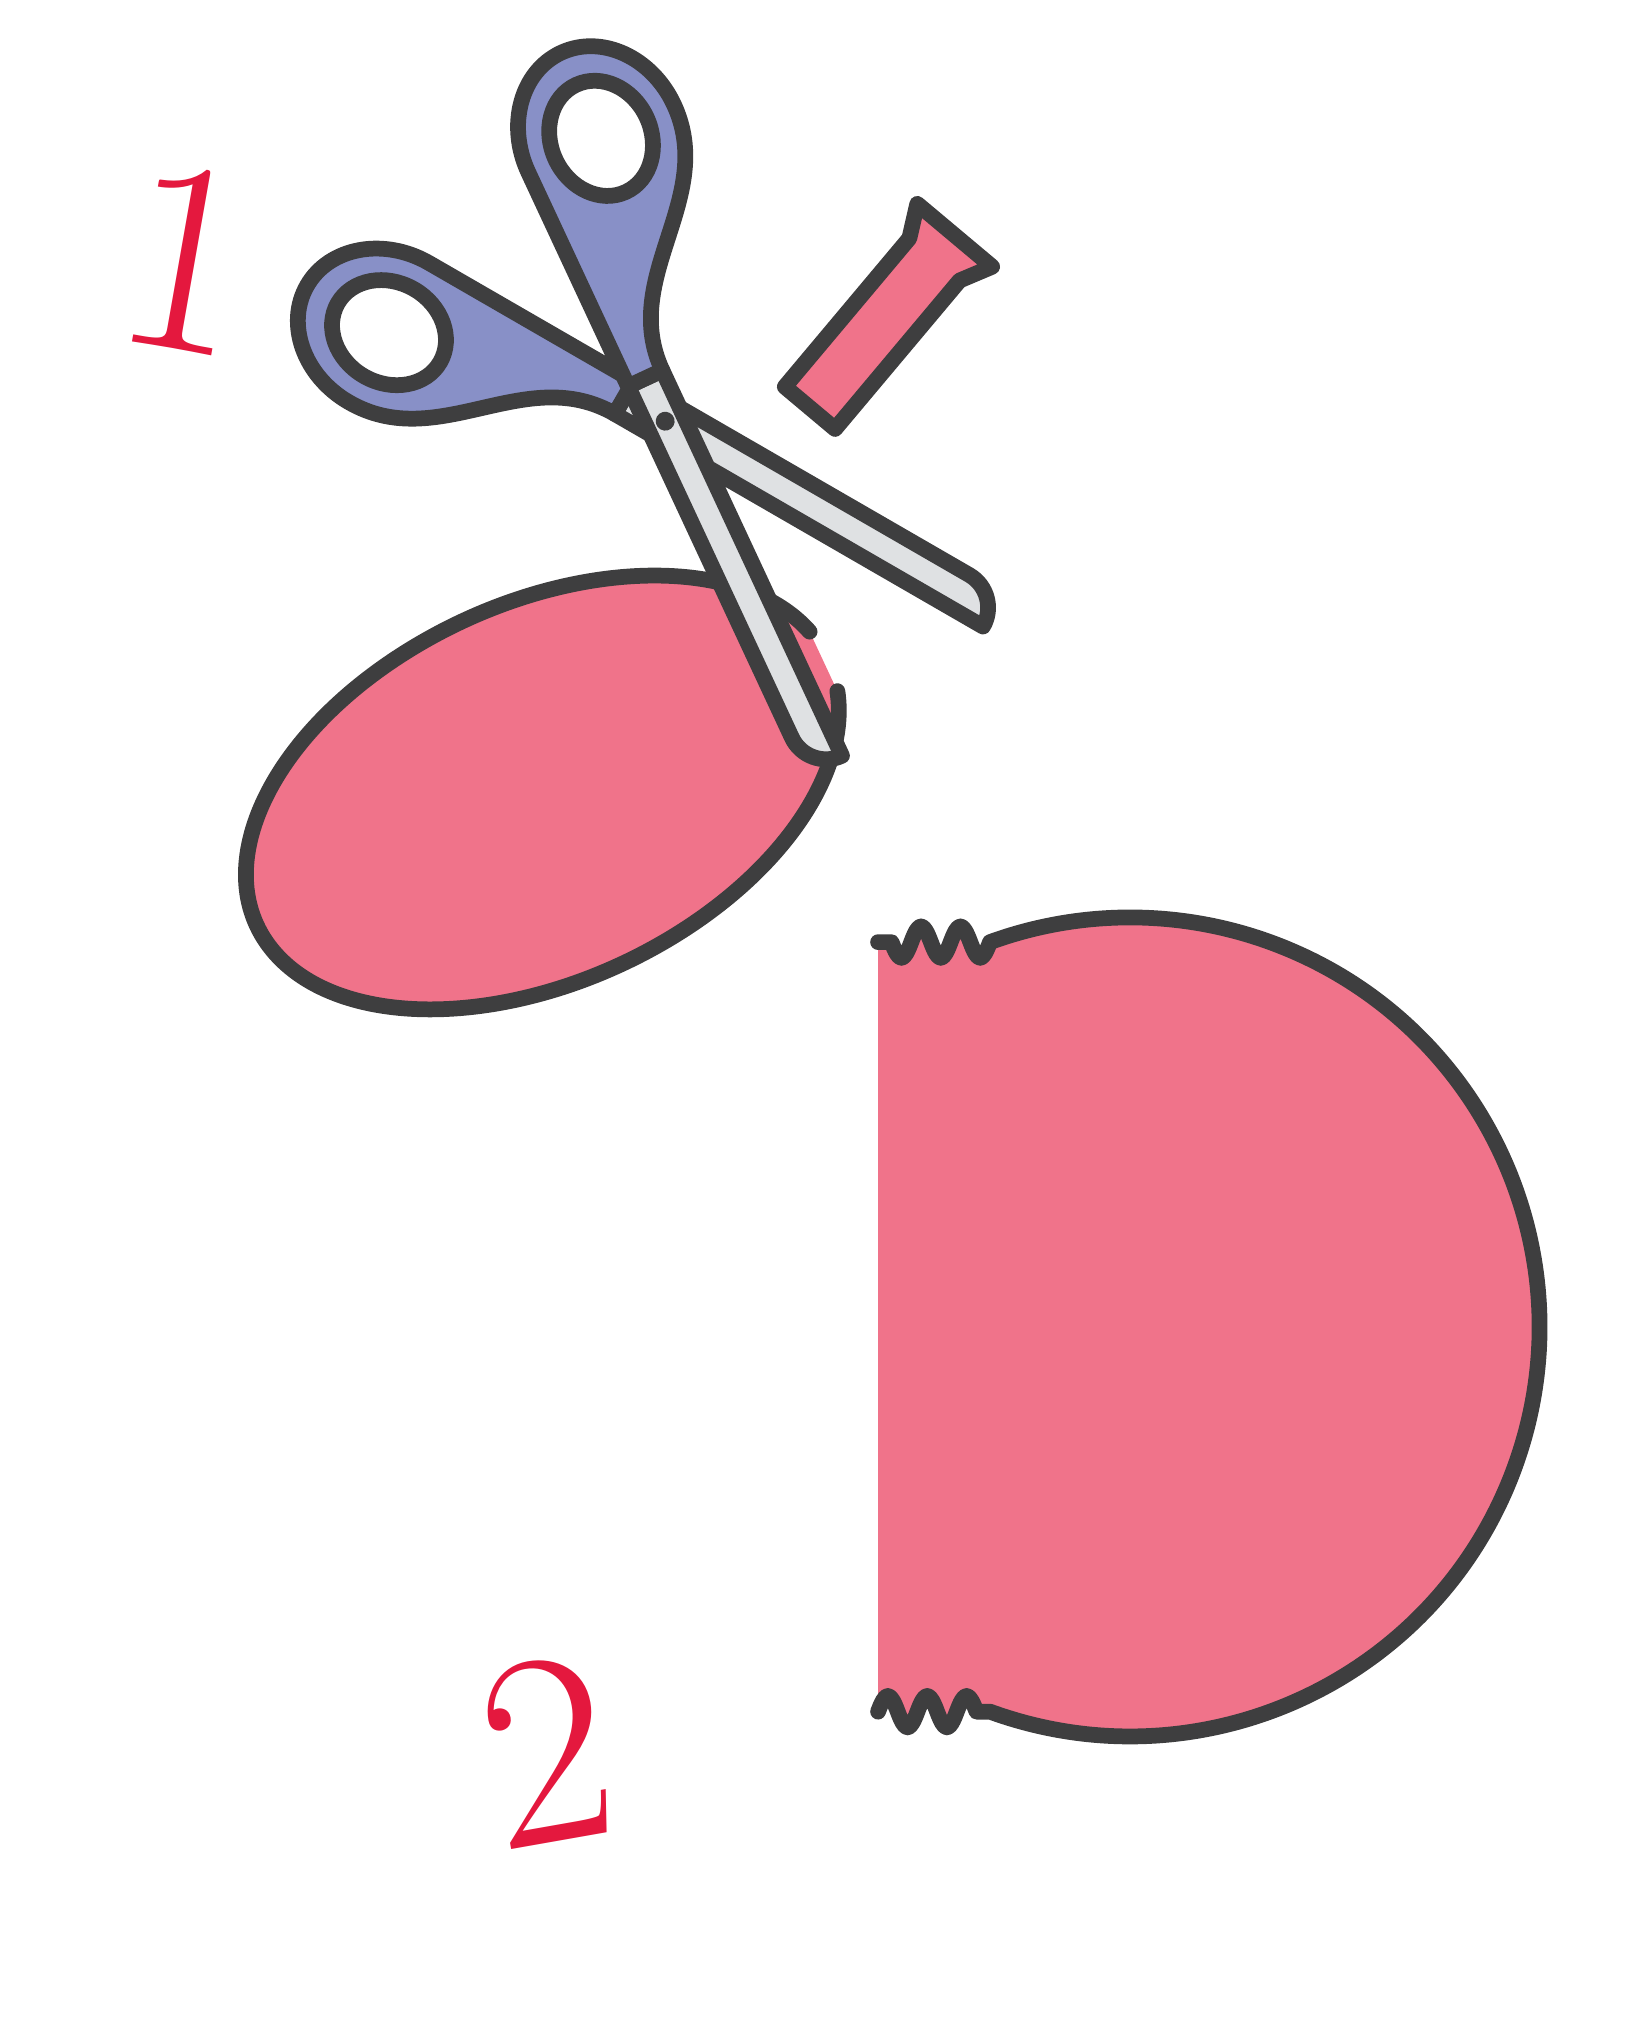
\begin{tikzpicture}[line join = round, line cap = round, line width = 2mm]%, decoration = {random steps, segment length = 3mm, amplitude = 0.5mm}]
    
    \begin{scope}[scale = 0.8, shift = {(-3,3)}, rotate = 15]
    \path[decorate, draw = ForegroundColour, fill = Red_3, rotate = 35, shift = {(2, 2)}]  
                                                   (15 :5 and 3 -| 8.5, 0) 
                                                -- (10 :5 and 3 -| 8  , 0) 
                                                % -- (10 :6 -| 7.5, 0) 
                                                % -- (350:6 -| 6.5, 0) 
                                                -- (10:5 and 3          ) 
                                                % arc (10:350:6      ) 
                                                -- (350:5 and 3)
                                                % -- (350 :6 -| 6.5, 0)
                                                % -- (350:6 -| 7.5, 0)
                                                -- (350:5 and 3 -| 8  , 0) 
                                                -- (345:5 and 3 -| 8.5, 0) 
                                                -- cycle;
    \path[decorate, draw = ForegroundColour, fill = Red_3, rotate = 10, shift = {(-1, 1)}]
                                                   (10:5 and 3) arc (10:350:5 and 3);


        \pgfmathsetmacro\bladewidth{0.4}
        \begin{scope}[scale = 0.75, shift = {(3, 8)}, rotate = -45]
            \path[decorate, draw = ForegroundColour, fill = ForegroundColour_5] (-1, -\bladewidth) to (8, -\bladewidth) arc (0:90:{2*\bladewidth*1cm}) -- (-1, \bladewidth) -- cycle;
            \path[decorate, draw = ForegroundColour, fill = ForegroundColour_5, yscale = -1, rotate = 35] (-1, -\bladewidth) to (8, -\bladewidth) arc (0:90:{2*\bladewidth*1cm}) -- (-1, \bladewidth) -- cycle;
            \path[decorate, fill = ForegroundColour] (0, 0) circle ({0.5*\bladewidth*1cm});
            \path[decorate, draw = ForegroundColour, fill = Accent3] (-1, -\bladewidth) to[out = 180, in = 0] (-6, -3) arc (270:90:2 and 1.7) -- (-1, \bladewidth) -- cycle (-6, {-1.5cm + 0.5 * \bladewidth * 1cm}) circle (1.25 and 1.0625);
            \path[decorate, draw = ForegroundColour, fill = Accent3, yscale = -1, rotate = 35] (-1, -\bladewidth) to[out = 180, in = 0] (-6, -3) arc (270:90:2 and 1.7) -- (-1, \bladewidth) -- cycle (-6, {-1.5cm + 0.5 * \bladewidth * 1cm}) circle (1.25 and 1.0625);
        \end{scope} 
    \end{scope}
                                                   \path[
                                                    draw = ForegroundColour, 
                                                    fill = Red_3, 
                                                    % fill opacity = 0.3, 
                                                    shift = {(4, -4)}, 
                                                    rotate = -90,
                                                    decoration = {
                                                        coil, 
                                                        aspect = 0, 
                                                        amplitude = 2mm, 
                                                        segment length = 5mm
                                                    },
                                                    scale = 0.8
                                                ]
                                                (-20:6.5 |- 0, -4) decorate {-- (-20:6.5)} arc (-20:200:6.5) decorate{-- (200:6.5 |- 0, -4)};

    \pgfresetboundingbox
    \useasboundingbox (-10, 12.5) rectangle (10, -12.5);
    \node[below right = 1cm, rotate = -10, Red, scale = 4] at (current bounding box.north west) {\Huge 1};
    \node[above left = 2cm, rotate = 10, Red, scale = 4] at (current bounding box.south) {\Huge 2};
\end{tikzpicture}
\end{document}